\chapter{Speaker Recognition Systems}

The process of voice recognition lies on the field of pattern classification, with the speaker and his or her utterance (a speech signal) as inputs for a classifier and a decision as output. This decision may be, given an utterance $\boldsymbol{Y}$ produced by a speaker $\mathcal{S}$ and a set $\boldsymbol{\mathcal{S}} = \{\mathcal{S}_1, ..., \mathcal{S}_S\}$ of known users,

\begin{equation}
    \mathcal{S} \gets \mathcal{S}_i \text{, if } i = \arg\max_j P(\mathcal{S}_j|\boldsymbol{Y}).
    \label{eq:decision_speaker_identification}
\end{equation}

\noindent This is a case of speaker identification and the output is a $\mathcal{S}_i$ from $\boldsymbol{\mathcal{S}}$. Another type of decision is

\begin{equation}
    \text{if } P(\mathcal{S}_i|\boldsymbol{Y}) \verifytest{\alpha}{\mathcal{S}}
    \label{eq:decision_speaker_verification}
\end{equation}

\noindent This is a speaker verification decision, with a binary output, given a $\mathcal{S}$ who produced $\boldsymbol{Y}$, a claimed identity $\mathcal{S}_i$ from $\boldsymbol{\mathcal{S}}$ and a threshold $\alpha$ for acceptance. This chapter (and indirectly the whole document) is about the type of decision from \equationref{decision_speaker_verification}.

\section{Basic Concepts}

\subsection{Utterance}

An utterance is a piece of speech produced by a speaker. It may be a word, a statement or any vocal sound. The terms \emph{utterance} and \emph{speech signal} sometimes are used interchangeably, but here speech signal will be associated to an utterance recorded and digitalized. An example of an utterance as speech signal is shown in \figureref{speech_signal}.

\begin{figure}[ht]
    \centering
    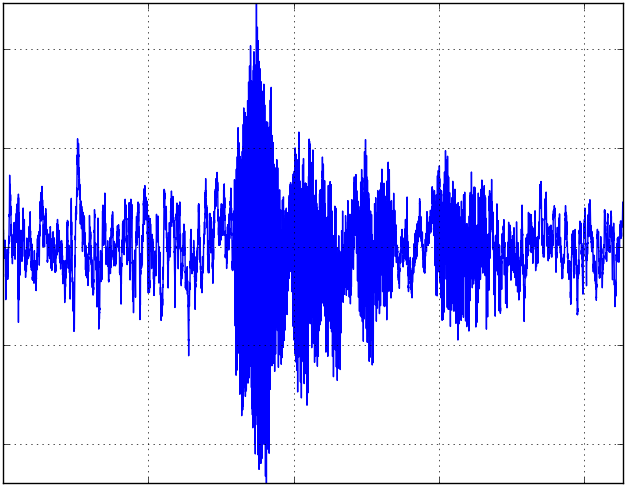
\includegraphics[width=\textwidth]{speech_signal}
    \caption{Speech signal for utterance ``karen livescu".}
    \label{fig:speech_signal}
\end{figure}

\subsection{Features}

The raw speech signal is unfit for usage by a recognition system. For a correct processing, the unique features from the speaker's vocal tract are extracted, reducing the number of variables the system needs to deal with (leading to a simpler implementation) and performing a better evaluation (just use the necessary informations). This extraction is executed by the MFCC algorithm, explained in \chapterref{feature-extraction}. Due to the stationary properties of the speech signal when analyzed in a short period of time, it is divided in overlapping frames of small and predefined length, to avoid ``loss of significancy" in the features \cite{davis.mermelstein.1980, rabiner.schafer.2007}.

\subsection{Dependency x Independency}

\section{Likelihood Ratio Test}

TODO basear-se na seção 2 do artigo ``Speaker Verification Using Adapted Gaussian Mixture Models".

\section{Basic Speaker Verification Architecture}

\subsection{Training Phase}

\subsection{Test Phase}